\documentclass[11pt]{article}
% Shared preamble for the Svetoch papers.
% Each paper.tex \input's this file (compile from inside the paper's folder):
%     \documentclass[11pt]{article}
%     % Shared preamble for the Svetoch papers.
% Each paper.tex \input's this file (compile from inside the paper's folder):
%     \documentclass[11pt]{article}
%     % Shared preamble for the Svetoch papers.
% Each paper.tex \input's this file (compile from inside the paper's folder):
%     \documentclass[11pt]{article}
%     \input{../tex/preamble.tex}
% Figures live in ../figures/*.pdf  (graphicspath set below).
\usepackage[utf8]{inputenc}
\usepackage[T1]{fontenc}
\usepackage{lmodern}
\usepackage[a4paper,margin=1in]{geometry}
\usepackage{amsmath,amssymb}
\usepackage{graphicx}
\graphicspath{{../figures/}}
\usepackage{booktabs}
\usepackage{caption}
\captionsetup{font=small,labelfont=bf}
% --- Minimal, siunitx-free unit support (so papers compile on any TeX install) ---
\usepackage{textcomp}
\newcommand{\SI}[2]{#1\,#2}
\newcommand{\si}[1]{#1}
\newcommand{\hertz}{Hz}
\newcommand{\meter}{m}
\newcommand{\centi}{c}
\newcommand{\milli}{m}
\newcommand{\micro}{\textmu}
\newcommand{\second}{s}
\newcommand{\kelvin}{K}
% ---------------------------------------------------------------------------------
\usepackage[colorlinks=true,linkcolor=blue,citecolor=blue,urlcolor=blue]{hyperref}
\usepackage{xcolor}
\definecolor{accent}{HTML}{6366F1}

% Common author block (add affiliation/ORCID if available before publishing)
\newcommand{\svetochauthor}{Oleg Yuryevich Kirichenko \\[4pt]
  \normalsize Independent researcher \\[2pt]
  \normalsize \href{mailto:urevich55@gmail.com}{urevich55@gmail.com} \quad\textbullet\quad GitHub: \href{https://github.com/infosave2007}{@infosave2007}}

\newcommand{\svetochfooter}{%
  \vspace{1em}\noindent\rule{\linewidth}{0.4pt}\\[2pt]
  {\footnotesize Part of the \emph{Svetoch} series (defensive publication, not patented).
  Project and code: \href{https://github.com/infosave2007/svetoch}{github.com/infosave2007/svetoch};
  related VMF/NVG theory: \href{https://github.com/infosave2007/vmf}{github.com/infosave2007/vmf}.
  Released for the public record to establish authorship and priority.}}

% Figures live in ../figures/*.pdf  (graphicspath set below).
\usepackage[utf8]{inputenc}
\usepackage[T1]{fontenc}
\usepackage{lmodern}
\usepackage[a4paper,margin=1in]{geometry}
\usepackage{amsmath,amssymb}
\usepackage{graphicx}
\graphicspath{{../figures/}}
\usepackage{booktabs}
\usepackage{caption}
\captionsetup{font=small,labelfont=bf}
% --- Minimal, siunitx-free unit support (so papers compile on any TeX install) ---
\usepackage{textcomp}
\newcommand{\SI}[2]{#1\,#2}
\newcommand{\si}[1]{#1}
\newcommand{\hertz}{Hz}
\newcommand{\meter}{m}
\newcommand{\centi}{c}
\newcommand{\milli}{m}
\newcommand{\micro}{\textmu}
\newcommand{\second}{s}
\newcommand{\kelvin}{K}
% ---------------------------------------------------------------------------------
\usepackage[colorlinks=true,linkcolor=blue,citecolor=blue,urlcolor=blue]{hyperref}
\usepackage{xcolor}
\definecolor{accent}{HTML}{6366F1}

% Common author block (add affiliation/ORCID if available before publishing)
\newcommand{\svetochauthor}{Oleg Yuryevich Kirichenko \\[4pt]
  \normalsize Independent researcher \\[2pt]
  \normalsize \href{mailto:urevich55@gmail.com}{urevich55@gmail.com} \quad\textbullet\quad GitHub: \href{https://github.com/infosave2007}{@infosave2007}}

\newcommand{\svetochfooter}{%
  \vspace{1em}\noindent\rule{\linewidth}{0.4pt}\\[2pt]
  {\footnotesize Part of the \emph{Svetoch} series (defensive publication, not patented).
  Project and code: \href{https://github.com/infosave2007/svetoch}{github.com/infosave2007/svetoch};
  related VMF/NVG theory: \href{https://github.com/infosave2007/vmf}{github.com/infosave2007/vmf}.
  Released for the public record to establish authorship and priority.}}

% Figures live in ../figures/*.pdf  (graphicspath set below).
\usepackage[utf8]{inputenc}
\usepackage[T1]{fontenc}
\usepackage{lmodern}
\usepackage[a4paper,margin=1in]{geometry}
\usepackage{amsmath,amssymb}
\usepackage{graphicx}
\graphicspath{{../figures/}}
\usepackage{booktabs}
\usepackage{caption}
\captionsetup{font=small,labelfont=bf}
% --- Minimal, siunitx-free unit support (so papers compile on any TeX install) ---
\usepackage{textcomp}
\newcommand{\SI}[2]{#1\,#2}
\newcommand{\si}[1]{#1}
\newcommand{\hertz}{Hz}
\newcommand{\meter}{m}
\newcommand{\centi}{c}
\newcommand{\milli}{m}
\newcommand{\micro}{\textmu}
\newcommand{\second}{s}
\newcommand{\kelvin}{K}
% ---------------------------------------------------------------------------------
\usepackage[colorlinks=true,linkcolor=blue,citecolor=blue,urlcolor=blue]{hyperref}
\usepackage{xcolor}
\definecolor{accent}{HTML}{6366F1}

% Common author block (add affiliation/ORCID if available before publishing)
\newcommand{\svetochauthor}{Oleg Yuryevich Kirichenko \\[4pt]
  \normalsize Independent researcher \\[2pt]
  \normalsize \href{mailto:urevich55@gmail.com}{urevich55@gmail.com} \quad\textbullet\quad GitHub: \href{https://github.com/infosave2007}{@infosave2007}}

\newcommand{\svetochfooter}{%
  \vspace{1em}\noindent\rule{\linewidth}{0.4pt}\\[2pt]
  {\footnotesize Part of the \emph{Svetoch} series (defensive publication, not patented).
  Project and code: \href{https://github.com/infosave2007/svetoch}{github.com/infosave2007/svetoch};
  related VMF/NVG theory: \href{https://github.com/infosave2007/vmf}{github.com/infosave2007/vmf}.
  Released for the public record to establish authorship and priority.}}


\title{\textbf{Computational Optics for Liquid Microsampling:\\
a Multi-Channel Smartphone Sensing Platform}\\[4pt]
{\large Svetoch Series, Paper V of VI}}
\author{\svetochauthor}
\date{17 June 2026}

\begin{document}
\maketitle

\begin{abstract}
\noindent We describe \textbf{MicroLab}, an application of the Svetoch method (Paper~I) that
turns an unmodified consumer smartphone into a multi-channel optical sensing platform for
liquid microsamples. The OLED screen is used both as a controllable structured light source
and --- through its built-in matrix polarizer --- as an opportunistic polarized source; the
camera is the detector and the cover glass an optical element. A microdroplet on a disposable
optical barrier is interrogated through three physically independent channels: \textbf{refractive}
(a dispersion index $D=C_r/C_b$, focal spread and edge contrast, with temperature-drift
correction; specific gravity, TDS, protein trends), \textbf{polarization} (Malus-law optical
rotation of chiral analytes), and \textbf{absorption} (RGB spectrophotometry against an
empty-lens baseline). A label-free \textbf{frustrated total internal reflection} mode uses the
cover glass as an evanescent-wave biosensor. The channels are fused into one repeatable
\emph{optical fingerprint}. The core contribution is a \textbf{validation discipline}: a
transfer-matrix self-QA gate (SVD rank/condition number) and a \textbf{Confidence Engine} that
\emph{rejects} a scan when signal is insufficient or droplet volume too small, instead of
guessing. MicroLab is \textbf{research-use / wellness-and-food-tech, not a validated medical
diagnostic}; medical claims (especially blood glucose) are explicitly \textbf{not} made.
\end{abstract}

\noindent\textbf{Keywords:} computational optics, smartphone diagnostics, refractometry,
mobile polarimetry, spectrophotometry, frustrated total internal reflection, sensor fusion,
confidence estimation, research-use-only.

\section{Introduction}
A modern smartphone packs, within millimetres, an emissive OLED display, an integrating
camera, and a precision cover glass. Papers~I--IV showed this hardware computes in light and
senses its own physics. Paper~V asks a practical question: can the same hardware extract a
repeatable optical fingerprint from a single microdroplet of liquid?

The honest framing matters. We do \emph{not} claim to ``measure everything'' in a drop; we
claim the narrower, defensible goal of extracting \textbf{stable, physically grounded optical
features} that are robust to droplet geometry and to hardware variability across phone models.
The platform is architected around three independent optical channels whose fusion yields a
fingerprint, plus a trust layer that knows when \emph{not} to report a number. This validation
discipline --- not any individual algorithm --- is the asset. We separate the platform into
trust tiers: food and technical liquids (zero regulatory risk), wellness trends, and regulated
medical claims (reserved for after clinical validation and cohort studies).
Figure~\ref{fig:microlab} shows the full signal stack.

\begin{figure}[ht]\centering
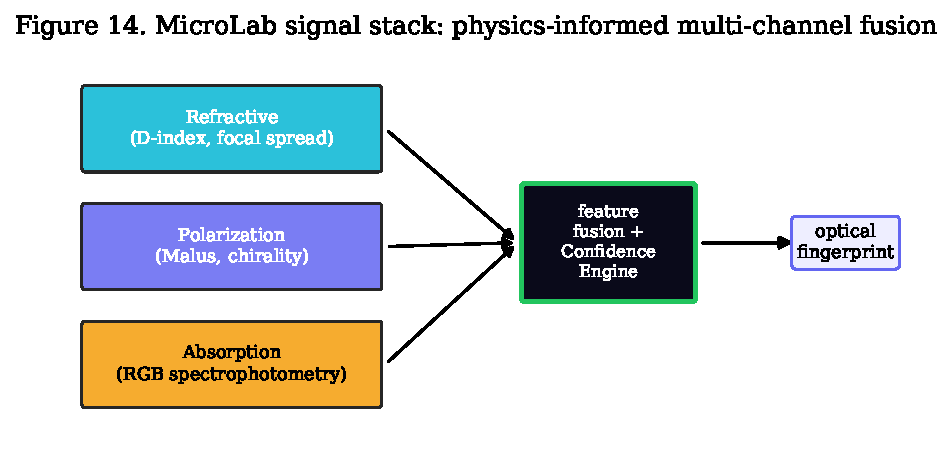
\includegraphics[width=0.92\linewidth]{fig14_microlab.pdf}
\caption{The MicroLab signal stack. Three physically independent channels --- refractive
(dispersion index, focal spread, edge contrast), polarization (Malus-law optical rotation),
and absorption (RGB spectrophotometry) --- feed a physics-informed feature-fusion layer
guarded by the Confidence Engine, producing one repeatable optical fingerprint of the
microdroplet.}
\label{fig:microlab}
\end{figure}

\section{The three-channel signal stack}
The technical core is sensor \textbf{fusion}, not a single trick; each channel reports
information the others cannot.

\subsection{Refractive mode --- dispersion index and interferometric path}
The screen--air-gap--cover-glass--camera path is a refractometer and, with reference fringes, a
Fabry--P\'erot interferometer. The primary engineered feature is a \textbf{dispersion index}
\begin{equation}
D = \frac{C_r}{C_b},
\end{equation}
the ratio of red- to blue-channel response of light traversing the droplet. Because refractive
index depends on wavelength and dissolved content, $D$ tracks specific gravity, total dissolved
solids and protein trends. Artefacts are averaged across multi-exposure and speckle patterns,
and a mandatory temperature-drift layer $D_\text{corr}=D-\kappa\,(T-T_0)$ removes thermo-optic
drift from local screen heating. For transparent media the Fabry--P\'erot fringe condition
\begin{equation}
2\,n\,d\,\cos\theta = m\,\lambda
\end{equation}
gives, for an index change $\Delta n$, a fringe-phase shift
$\Delta\phi = (4\pi d\cos\theta/\lambda)\,\Delta n$, measured to sub-pixel precision against
the displayed reference pattern --- optical density / concentration with no moving parts.

\subsection{Polarization mode --- Malus-law optical rotation}
OLED panels carry a built-in polarizer to suppress ambient reflection, so emitted light is
partially polarized; MicroLab treats it as a \textbf{free, opportunistic polarized source}.
Analysing the angle-dependent intensity follows Malus's law,
\begin{equation}
I(\theta) = I_0 \cos^2(\theta - \alpha),
\end{equation}
where $\alpha$ is the optical rotation of a chiral analyte. Fitting $\alpha$ versus path length
and concentration yields a saccharimetry-style readout (sugars, glucose as R\&D only),
positioned as a research module providing a differentiation boost.

\subsection{Absorption mode --- RGB spectrophotometry}
The OLED is a controllable RGB backlight and the camera a three-band photometer, applying the
Beer--Lambert law,
\begin{equation}
A_\lambda = -\log_{10}\!\frac{I_\lambda}{I_{0,\lambda}} = \varepsilon_\lambda\, c\, \ell ,
\end{equation}
with $I_{0,\lambda}$ the intensity through an \textbf{empty-lens baseline}. Green-channel
absorption tracks blood-like samples (haemoglobin); blue-channel attenuation tracks urine
chromophore trends (urobilin). Baseline normalization makes the channel robust to backlight
ageing and exposure changes.

\section{Label-free frustrated-TIR sensing}
A fourth, label-free modality uses the cover/prism glass as an \textbf{evanescent-wave
biosensor}. Display light is coupled above the critical angle $\theta_c=\arcsin(n_2/n_1)$ for
total internal reflection; the evanescent field extends a fraction of a wavelength into the
sample. An analyte contacting the surface \textbf{frustrates} the reflection, and the reflected
contrast/interference pattern read by the camera changes with the local refractive index and
surface binding. Scanning the fringe period and recording the peak contrast ratio gives a
quantitative response. Being interface- rather than bulk-sensitive, this mode complements the
refractive and absorption channels and opens a route to surface-binding assays. The audit rates
it (A3) as strong; it is disclosed here defensively as part of the open fingerprint stack.

\section{Sensor self-QA by transfer-matrix SVD}
No measurement is trustworthy without a metrology gate. Before any droplet, MicroLab
characterizes the display$\to$lens$\to$sensor chain. Dark (null) frames and calibration
patterns measure leakage and display$\to$sensor cross-talk; one-hot display patterns build an
empirical transfer matrix $\mathbf{M}$, whose singular-value decomposition
\begin{equation}
\mathbf{M} = \mathbf{U}\,\boldsymbol{\Sigma}\,\mathbf{V}^{\!\top}
\end{equation}
yields the \textbf{rank} and \textbf{condition number}
$\kappa=\sigma_\text{max}/\sigma_\text{min}$ --- quantitative metrics of vignetting and optical
degradation. A degraded or contaminated lens collapses the small singular values, raising
$\kappa$ and lowering the effective rank, and the channel is flagged unfit. This is the
\textbf{``Auto-Air'' quality gate}: an automatic baseline-aberration check run on air, before
the sample, that must pass before measurement begins. Rated (B3) moderate; its value is
operational --- the first line of the validation discipline.

\section{Feature fusion and the Confidence Engine}
The channels do not vote in isolation. Physically grounded features --- $D$ and $D_\text{corr}$,
focal spread, edge/structure contrast and standard deviation, the Malus rotation angle, per-band
absorbances, and the frustrated-TIR contrast peak --- are \textbf{fused} into one feature
vector. The strategy is conservative: physics-informed engineered features first, a supervised
model only on top, never raw pixels into a black box. The decisive component is the
\textbf{Confidence Engine}, a trust layer that scores every scan and \textbf{rejects} it when
evidence is inadequate (low SNR, too small a droplet, failed Auto-Air, cross-channel
inconsistency). The product is expected to say \emph{``not enough data, please re-scan''} rather
than guess, and every result carries an explicit status (\emph{estimated}, \emph{trend-only},
\emph{needs lab confirmation}). This honesty discipline is the moat: the contribution is the
rejection logic and physically grounded fusion (A4, strong), not the classifier.

\section{Measurement map and use-cases}
The platform is built bottom-up, from low-regulation, easy-ground-truth scenarios toward
medical trust (Table~\ref{tab:map}).

\begin{table}[ht]\centering\small
\caption{Measurement map: targets, status and claim level.}
\label{tab:map}
\begin{tabular}{llll}
\toprule
Target & Status & Why promising & Claim level\\
\midrule
Urine specific gravity & Strong MVP & Direct refractive link; minimal prep & Wellness $\to$ clinical (after validation)\\
Coffee TDS / Brix (food) & Strong MVP & Zero regulatory risk; fast loop & Food-tech, immediate\\
Total serum protein & Research candidate & Strong optical tradition & Research-use-only\\
Saliva fertility (ovulation) & Conditional & Large consumer interest & Trend-assistance only\\
Tear osmolarity trend & Conditional & Niche premium market & Trend-only, later-stage\\
Blood glucose & High-risk R\&D & Large market & \textbf{No claim} --- R\&D only\\
\bottomrule
\end{tabular}
\end{table}

The strongest first products carry no medical risk: coffee TDS/Brix and water checks deliver
revenue and diverse cross-device data immediately. Urine specific gravity is the natural bridge
to a future clinical pilot (direct refractive link; cheap gold-standard refractometer). Blood
glucose is retained only as an open research hypothesis with \textbf{no diagnostic claim}.

\section{Methods}
\textbf{Hardware:} reference device Xiaomi 12 Lite (6.55" AMOLED, $2400\times1080$,
\SI{120}{\hertz}; 32\,MP camera; built-in display polarizer; cover glass as TIR/refractive
element). A disposable \textbf{optical barrier strip} sets sterility and a repeatable optical
stack over the lens. \textbf{Ritual:} (1)~apply barrier; (2)~run the Auto-Air SVD gate before
the droplet; (3)~apply the droplet with an on-screen volume guide; (4)~burst-capture while the
screen emits the channel pattern sequences (refractive gradients, polarization sweep, RGB
photometry, TIR fringe scan); (5)~fuse features, run the Confidence Engine, report with status;
(6)~remove and discard the barrier. \textbf{Calibration / ground truth:} each mode has an
external reference (refractometer, TDS meter, lab assay); datasets log phone model, screen type,
ambient light, temperature, film thickness, and timestamped repeats for drift. \textbf{Software:}
built on the Svetoch on-device stack (Paper~I).

\section{Discussion: hard truths}
\textbf{Confounders as measurable nuisance variables.} Sample inhomogeneity, ambient-light
leakage, barrier-film microcracks and local screen overheating are real; MicroLab treats them
as measurable nuisance variables handled by quality gates (multi-exposure/speckle averaging,
empty-lens baseline, Auto-Air, temperature-drift correction). Unbounded confounders trigger a
rejection. \textbf{Regulatory tiers.} Claims are split into \emph{educational}, \emph{wellness},
\emph{research-use-only}, and \emph{regulated diagnostic}; the first three are available now, the
last reserved strictly for after clinical validation and cohort studies (planned pilot: urine
specific gravity in a clinic). \textbf{Explicit non-medical claims.} MicroLab as described is
\textbf{not a validated medical diagnostic}; no diagnostic claim is made for any biofluid, and
blood glucose is explicitly excluded from any present claim. The contribution is the
\emph{honesty and confidence discipline} --- a system that refuses to guess. \textbf{Patent
context:} the audit rates polarimetry (A2), frustrated-TIR (A3) and multimodal fusion with the
Confidence Engine (A4) as strong, and the interferometer/refractometer (B2) and sensor self-QA
(B3) as moderate; all are disclosed openly here.

\section{Conclusion}
A smartphone can be a multi-channel optical sensing platform. Combining a refractive dispersion
channel, an opportunistic Malus-law polarization channel, RGB absorption spectrophotometry, and
label-free frustrated-TIR sensing, MicroLab extracts a repeatable optical fingerprint from a
single microdroplet. Guarded by a transfer-matrix self-QA gate and a Confidence Engine that
rejects untrustworthy scans, it is honest about what it can and cannot measure. The validation
discipline --- not the machine learning --- is the contribution, and the medical tier remains
explicitly off-limits until clinical validation.

\paragraph{Data and code.} \href{https://github.com/infosave2007/svetoch}{github.com/infosave2007/svetoch}; related VMF/NVG theory: \href{https://github.com/infosave2007/vmf}{github.com/infosave2007/vmf}
(Apache-2.0).
\paragraph{Priority note.} Released as a defensive publication to establish authorship and date
of disclosure; the author has elected not to seek patent protection.

\begin{thebibliography}{9}\small
\bibitem{edlen} B. Edl\'en, ``The refractive index of air,'' \emph{Metrologia} \textbf{2}, 71 (1966).
\bibitem{hecht} E. Hecht, \emph{Optics}, 5th ed., Pearson, 2017 (Malus's law; polarimetry/saccharimetry).
\bibitem{beer} D. F. Swinehart, ``The Beer--Lambert law,'' \emph{J. Chem. Educ.} \textbf{39}, 333 (1962).
\bibitem{fan} X. Fan et al., ``Sensitive optical biosensors for unlabeled targets: a review,'' \emph{Anal. Chim. Acta} \textbf{620}, 8 (2008).
\bibitem{ozcan} A. Ozcan and E. McLeod, ``Lensless imaging and sensing,'' \emph{Annu. Rev. Biomed. Eng.} \textbf{18}, 77 (2016).
\bibitem{golub} G. H. Golub and C. F. Van Loan, \emph{Matrix Computations}, 4th ed., Johns Hopkins, 2013 (SVD / system characterization).
\end{thebibliography}

\svetochfooter
\end{document}
